29. $y=\cfrac{x^2-4x+3}{|x-3|}=\cfrac{(x-3)(x-1)}{|x-3|}=\begin{cases} x-1,\ x>3,\\ 1-x,\ x<3.\end{cases}.$
$$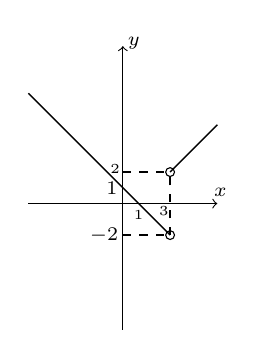
\begin{tikzpicture}[scale=0.2]
\tikzset {line01/.style={line width =0.5pt}}
\tikzset{line02/.style={line width =1pt}}
\tikzset{line03/.style={dashed,line width =0.5pt}}
%\filldraw [black] (0,0) circle (1pt);
\draw [->] (-6,0) -- (6,0);
\draw [->] (0,-8) -- (0,10);
\draw[line01] (-6,7) -- (3,-2);
\draw[line01] (3,2) -- (6,5);
\draw[line03] (3,-2) -- (3,2);
\draw[line03] (0,2) -- (3,2);
\draw[line03] (0,-2) -- (3,-2);
\draw (6.2,0.7) node {\scriptsize $x$};
\draw (-1.2,-2) node {\scriptsize $-2$};
\draw (-0.7,1) node {\scriptsize $1$};
\draw (-0.5,2.2) node {\tiny $2$};
\draw (1,-0.7) node {\tiny $1$};
%\draw (-0.7,3) node {\tiny $3$};
\draw (2.6,-0.5) node {\tiny $3$};
%\draw (3.2,-0.7) node {\tiny $3$};
\draw (0.7,10.2) node {\scriptsize $y$};
\draw (3,-2) circle (8pt);
\draw (3,2) circle (8pt);
\end{tikzpicture}$$
